% q3_abcd.tex - Question 3 Studies A-D (OWNER: B) - prose integrated verbatim from docs/B_Q3_ABCD.md
\section{Question 3, Studies A--D}

All tests are two-sided with $\alpha = 0.05$ and 95\% confidence intervals. Every test call is the version taught in the course slides (Weeks 6--8). Each study keeps the full set of records defined by the assignment's own filtering code, and the four studies answer their own questions: Study A and B target population means, Study C a sign probability, Study D whole distributions --- the four are not interchangeable conclusions.

\subsection*{Study A --- Is there a league salary gap?}

\textbf{Design.} The response is the natural log of 1987 salary, a quantitative variable; the two leagues are independent groups. Of 322 players, 59 have missing salaries and none has a non-positive salary, leaving $n = 139$ American and $n = 124$ National. $\Hnull$: the two population mean log salaries are equal; $\Halt$: they differ.

\textbf{Method.} Shapiro--Wilk rejects normality in both groups ($W = 0.974$, $\pval = 0.009$; $W = 0.962$, $\pval = 0.002$), but both samples are large (Week 6: $n \geq 30$, CLT) and the question asks about the population \emph{mean}, so a two-sample t-test is the course method here. The Week 7 F-test for equal variances gave $F(138, 123) = 1.031$, $\pval = 0.867$, so there is no evidence against equal variances and the pooled t-test is used.

\textbf{Result.} $t(261) = 0.104$, $\pval = 0.917$, 95\% CI for the difference in means $[-0.205,\ 0.228]$. Group means are nearly identical (5.933 vs 5.921). We fail to reject $\Hnull$: the data provide no evidence of a league gap in mean log salary. On the salary scale the interval corresponds to a multiplicative factor between about 0.81 and 1.26, so a practically meaningful gap in either direction is not supported either.

\begin{figure}[htbp]
  \centering
  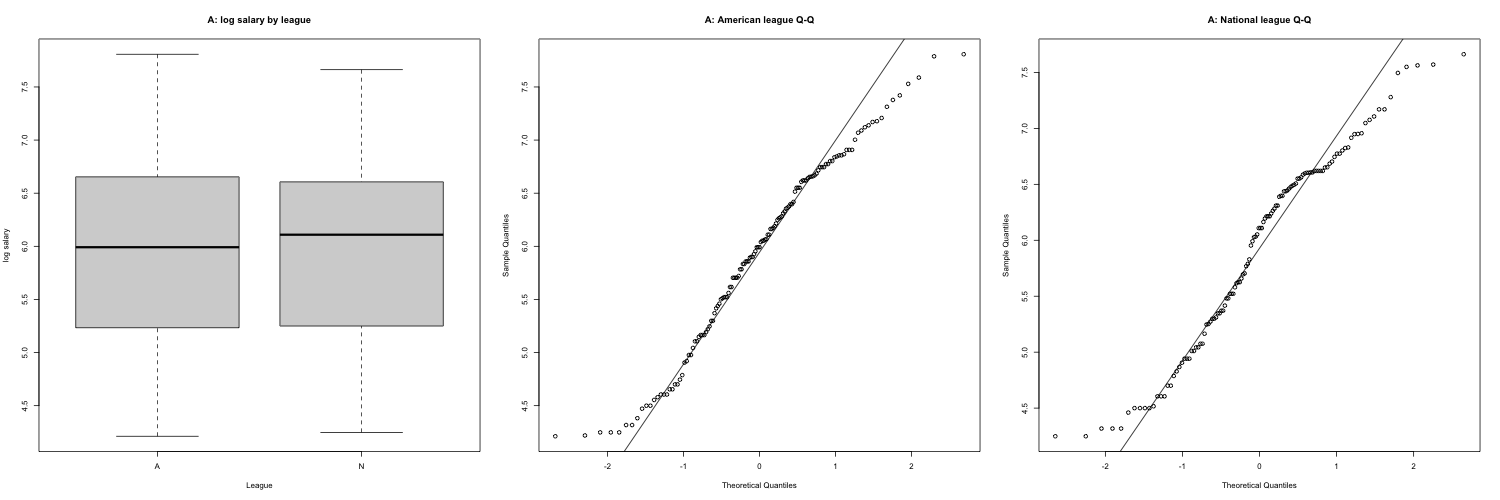
\includegraphics[width=\textwidth]{Q3_A_diagnostics.png}
  \caption*{Study A diagnostics: boxplot and Q--Q plots.}
\end{figure}

\subsection*{Study B --- Tuition versus living costs}

\textbf{Design.} Each college contributes both measurements, so the design is paired; all 777 colleges are retained (no missing or non-positive values). The response is the difference $\log(\text{Outstate}) - \log(\text{Room.Board})$. $\Hnull$: the population mean difference is zero; $\Halt$: it is not.

\textbf{Method.} Following the Week 8 pattern, the differences were checked first: Shapiro--Wilk rejects strict normality ($W = 0.987$, $\pval < 0.001$), but with 777 pairs ($n \geq 30$, CLT) and a mean-difference question, the Week 7 paired t-test is the course method.

\textbf{Result.} The mean log difference is 0.828 (SD 0.304), $t(776) = 75.774$, $\pval < 0.001$, 95\% CI $[0.806,\ 0.849]$. We reject $\Hnull$. Out-of-state tuition is clearly the larger bill: $\exp(0.828) \approx 2.29$, so tuition is on average about 2.3 times room-and-board costs, with the interval corresponding to factors from 2.24 to 2.34.

\begin{figure}[htbp]
  \centering
  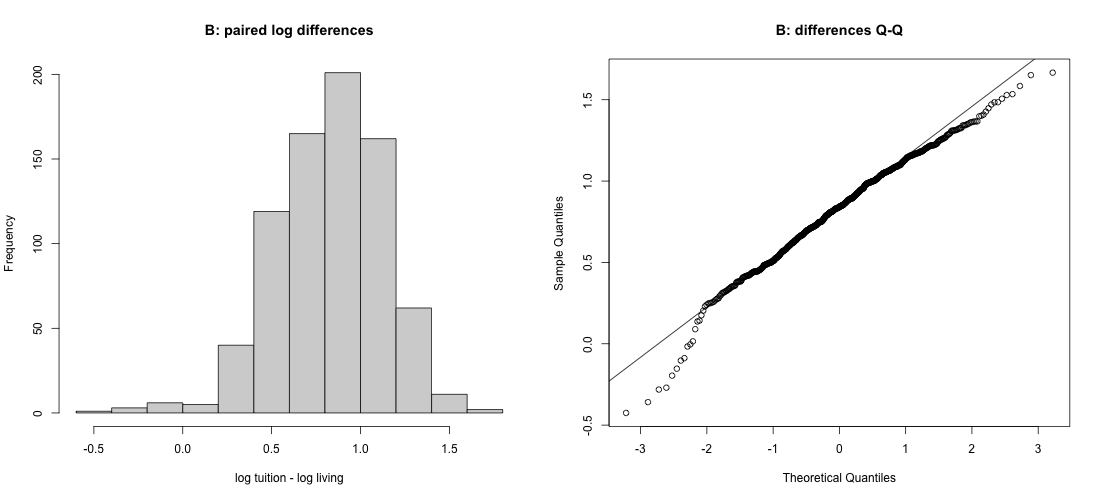
\includegraphics[width=0.9\textwidth]{Q3_B_diagnostics.png}
  \caption*{Study B diagnostics: histogram and Q--Q plot of the paired differences.}
\end{figure}

\subsection*{Study C --- Which bill is more often larger?}

\textbf{Design.} Same 777 colleges, but only the sign of Outstate $-$ Room.Board matters: 767 positive, 10 negative, 0 ties. $\Hnull$: among colleges where the two costs differ, $P(\text{tuition} > \text{room-and-board}) = 0.5$; $\Halt$: the probability differs from 0.5.

\textbf{Method.} This is a sign test, done with the Week 6 one-sample proportion test \texttt{prop.test(x, n, p = 0.5)}. It uses only the counts of positive and negative differences, so it assumes nothing about the shape of the cost distributions --- exactly what the question requires.

\textbf{Result.} $\hat{p} = 0.987$, 95\% CI $[0.976,\ 0.993]$, $\chisq(1) = 735.570$ with continuity correction, $\pval < 0.001$. We reject $\Hnull$: at almost every college, tuition is the larger bill. An exact binomial test was run as a cross-check and gives the same decision, but the course method is what is reported here.

\textbf{Compared with Study B.} Study B asks how large the gap is on average (a mean log difference); Study C asks only which side is larger (a probability). The two can disagree in principle --- a large-but-balanced gap would make B significant and C not --- but here they agree: tuition is both consistently the larger bill and much larger on average. C says nothing about magnitude, B says nothing about consistency; together they describe the gap fully.

\subsection*{Study D --- American versus Japanese fuel economy}

\textbf{Design.} mpg is quantitative; the two origin groups are independent ($n = 245$ American, $n = 79$ Japanese; all 324 retained cars have valid mpg). $\Hnull$: the two mpg distributions are identical; $\Halt$: they differ.

\textbf{Method.} Week 8 flow: Shapiro--Wilk per group rejects normality for American cars ($W = 0.934$, $\pval < 0.001$), so the two-sample t-test is not appropriate for comparing distributions; the Mann--Whitney U test (Wilcoxon rank-sum) is used instead. mpg contains tied values, so R automatically uses the normal approximation of W with continuity correction.

\textbf{Result.} $W = 2456.5$, $\pval < 0.001$. We reject $\Hnull$: the distributions differ. Japanese cars have systematically higher fuel economy --- median 31.6 mpg (IQR 8.4) versus 18.5 (IQR 9.0) for American cars. As in any observational comparison of groups, this is a difference between the cars in this 1993-era dataset, not an effect of origin itself.

\begin{figure}[htbp]
  \centering
  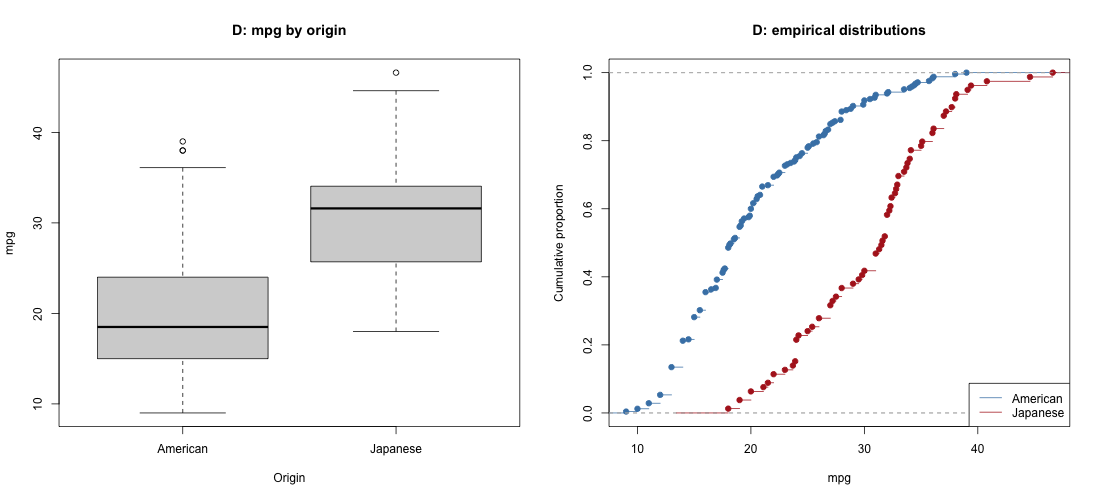
\includegraphics[width=0.9\textwidth]{Q3_D_distributions.png}
  \caption*{Study D diagnostics: boxplot and empirical CDFs.}
\end{figure}
